\chapter{Implementation}
\label{chp:implementation}

\par The research this thesis presents relies on a custom \ac{IP} address hopping solution. This chapter covers many of the details of this system, from high-level architecture to the network protocol. Section \ref{sec:arg_requirements} covers the requirements this system strives to meet. Section \ref{sec:arg_impl_overview} gives an architecture overview, while Section \ref{sec:arg_components} covers the details of each component in the system. Section \ref{sec:arg_protocol} details the network protocol used by the system to coordinate gateways.

\section{Requirements}
\label{sec:arg_requirements}
\par \ac{ARG} focuses on the needs of military networks. These are essentially the needs of any geographically-diverse organization: locations throughout the world, high availability and reliability requirements, and security over any network through which its data travels \cite{DialInNetworking}.

\par ARG primarily attempts to protect communication outside of military-controlled networks and prevent external entities from probing internally. This protection includes privacy, as \ac{ARG} (like any network address space randomization tool) helps hide information from adversaries by obfuscating sender and receiver information \cite{NetworkBasedPrivacy}. This means that the implementation described is intended to be employed for all traffic traveling between bases, but is unconcerned with internal base traffic. Internal network defense remains the purview of traditional defenses. Base networks, in this case, include both those on permanent installations and those in deployed, forward locations. 

\par ARG must operate over the commercial Internet. Some proposals for network address space randomization require changes to the Internet's existing routing infrastructure and protocols \cite{CONTRA, APOD}. Deploying such a solution may be possible and beneficial in the long run, but a solution that could be deployed today without participation from outside entities is more feasible. This is especially true for forward locations, where traffic is more likely to utilize infrastructure outside the military's control.

\par Like any large, distributed organization, bases can generate huge volumes of traffic, so ARG must scale well. Due to the importance of networks to command and control, ARG's implementation must not introduce significant latency under any foreseeable load. Likewise, there can never be a brief period where all connections drop. At a minimum, given the number of nodes inside the network, dropped connections result in a massive amount of wasted bandwidth as they are reestablished and the data retransmitted.

\par Military networks contain a wide range of hardware and software. Much of this software cannot be altered to accommodate \ac{ARG}, so it must function transparently. Host-level implementations might be feasible for generic workstation images (i.e., an alteration to the operating system's network stack), but the ability to function in another way must exist to allow legacy equipment to continue operating.

%\par Finally, resource constraints---monetary and manpower---preclude some options. ARG is intended to be easily configurable and usable with reasonable hardware investments. ARG requires only a single gateway system for each network it is intended to protect, rather than hardware and/or software for every client inside those networks.

\section{Architecture Overview}
\label{sec:arg_impl_overview}
%\par Based on these requirements and the previously cited literature, this paper proposes the Address Routing Gateway. While actual testing of this setup is beyond the scope of this paper, we will attempt to analyze the advantages it would provide, based on previous experimentation.

\par As illustrated in Figure \ref{fig:arg_concept_network}, \ac{ARG} functions entirely around standard networks with hopping gateways. This matches the ``gateway hopping'' scheme discussed in Section \ref{sec:gateway_hopping}. As with \cite{TAO}, these gateways are standalone systems, not intended for use with other tasks. Individual hosts inside these networks have no knowledge of the traffic transformations the gateways perform, whether their connections are routing to a host inside the local network, to a host inside another associated hopping network (hereafter referred to as an ``ARG network''), or to an external network. The implementation of ARG allows the deployment of standard passive defense technologies like firewalls inside the network without reconfiguration. Each gateway maintains a \ac{NAT}-like table to ensure that existing connections are maintained across hops (essentially temporarily leaving the old IP active for just those connections using it already).

\begin{figure}
	\centering
	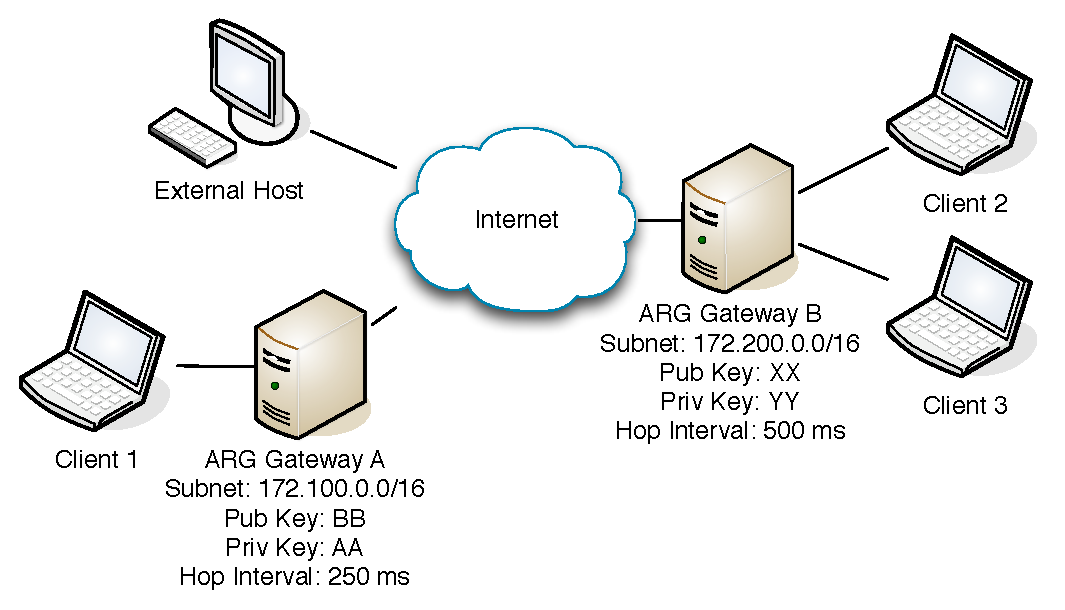
\includegraphics[width=1\textwidth]{arg_concept_network}
	\caption{\ac{ARG} conceptual network layout}
	\label{fig:arg_concept_network}
\end{figure}

\par Each gateway is given what subnet it is permitted to hop within, a private/public key pair, and time it should wait between \ac{IP} address changes (frequently referred to as its ``hop interval''). For example, \ac{ARG} Gateway A in Figure \ref{fig:arg_concept_network} uses subnet 172.100.0.0/16, has the specified public and private keys, and hops every 250 milliseconds. Additionally, each gateway is pre-configured with knowledge of at least one other gateway. The configured information consists solely of the subnet the other gateway is handling and a public key to use for authentication with it. In the figure, this would mean that Gateway A knows that Gateway B sits in the 172.200.0.0/16 subnet and has the public key XX, but nothing else. The gateways transfer additional information during the connection process. 

\par At startup, each gateway generates a random symmetric encryption key and a ``hop key.'' They then attempt to connect to all other gateways for which they have configuration files through a series of data and time synchronization packets. Once two gateways fully connect, they exchange data about all other gateways they have configured, allowing \ac{ARG} nodes to connect to gateways for which they do not have physical configuration files. Periodically gateways re-send time synchronization information, ensuring that changing network conditions do not kill communication. Section \ref{sec:arg_protocol} and Appendix \ref{chp:protocol} cover each of these packet exchanges in more detail.

\par Once connected, packets between ARG networks are encapsulated, encrypted, and authenticated by the originating network's gateway, with each packet given the destination network's current \ac{IP} address. On receipt, a gateway checks that the \acp{IP} match what they expect (both its own IP and the source's IP), then validates the authentication information (signature/\ac{HMAC}) before forwarding the original packet into their network. \acp{IP} may match either the current address or the previous one, allowing packets sent just before an \ac{IP} change to still be accepted. Packets to external hosts flow through the \ac{NAT}-style system covered in Section \ref{sec:arg_nat}. 

%\par Multi-homed networks are not taken into account in this proposal. Further research is needed to see what changes would need to be made to support this setup. If an ARG gateway were placed at each of the connections to the outside network, it is likely that some communication between the two is required to keep them working together \cite{SandiaDynat}, but the exact form this would take needs consideration. \tbd{move to limitations?}

\section{Components}
\label{sec:arg_components}
The handling of packets within ARG is distinctly different if they are to an external (non-ARG network) host or to an ARG network. These processes are handled by two separate components, the hopper and the NAT. A high-level director decides which of these two receives each incoming packets. All of these components run as separate threads on the same gateway, closely coordinating their work. Because it is in charge of overall system operation, this section begins by discussing the director.

\subsection{Director}
\label{sec:arg_director}
\par The director is in charge of receiving packets on the internal and external interfaces of the gateway. Upon receipt of a packet, the director parses the packet and decides how to handle it. The director's decision tree is illustrated in Figure \ref{fig:arg_director_flow} and discussed below.

\begin{figure}
\caption{\ac{ARG} director flow}
\label{fig:arg_director_flow}
\centering
\includegraphics[width=1.0\textwidth,clip=true,trim=0 0 0 0]{flow_director}
\end{figure}

\par In the case of \ac{ARP} requests on either interface, the director replies with the gateway's \ac{MAC} address. This feature of \ac{ARG} allows its use without any changes to the network it is placed in, as hosts continue to send to the ``same'' gateway IP as before and \ac{ARG} responds, despite not technically possessing an internal \ac{IP} of its own. For example, the inside hosts send out an \ac{ARP} request for their normal \ac{IP} gateway (as Section \ref{sec:eth_routing} discusses) and the \ac{ARG} gateway sends an \ac{ARP} response, allowing it to grab all traffic and process it appropriately. More details on Ethernet and \ac{IP} routing can be found in Sections \ref{sec:eth_routing} and \ref{sec:ip_routing}.

\par For outgoing packets (packets that are sent from within the protected network that are intended to leave the network), the director checks the destination \ac{IP} of the packet. If the IP is unknown, it is passed to the \ac{NAT} module. If the IP is within another \ac{ARG} network the director knows, the packet is handed off to the hopper module to be wrapped and transmitted.

\par For incoming packets (packets hitting the external interface), the director first checks if the source IP is another ARG network. If it is \textit{not}, the director quickly hands the packet off to the NAT inbound handler.

\par If the packet \textit{is} from another ARG network, the director checks if the packet type indicates it is an administrative packet and hands it off to the hopper's administrative processor. If it is not an administrative packet, the director confirms the gateway the packet is from is actually connected. Which gateway is determined by matching the source \ac{IP} to the base \ac{IP} and mask in the local gateway's configuration. Assuming that the gateway is connected, the local gateway checks that the source and destination \acp{IP} are correct, based on the data the hopper has on the other gateway. Assuming all checks pass, the packet is handed off to the hopper to be unwrapped and forwarded into the network. If any fail, the packet is silently dropped.

\subsection{Hopper}
\label{sec:arg_hopper}
\par The hopping module is the heart of ARG. It maintains the state of the gateways (e.g., keys, hop intervals, times) it knows about and transfers packets to and from the network it is protecting. The other two components (director and \ac{NAT}) talk to the hopper to obtain current IP information and if a given gateway is connected or not. 

\par When the hopper first starts, it initializes a list of gateways with data from configuration files. The information maintained in this structure is shown in Table \ref{tab:gatestate}. 

\begin{table}
\caption{Information hopper module maintains on other \ac{ARG} gateways}
\label{tab:gatestate}
\centering
\begin{tabular}{l|l}
	\textbf{Data} & \textbf{Information Source}\\
	\hline
	IP Range (IP and mask) & Configuration file (see Appendix \ref{chp:argconf})\\
	\ac{RSA} Public Key & Configuration file\\
	Hop Interval & Transferred during connection (see Section \ref{sec:arg_protocol})\\
	Symmetric Key & Transferred during connection\\
	Hop Key & Transferred during connection\\
	Time Base & Calculated based on latency\\
\end{tabular}
\end{table}

\par An administrative thread is started at the same time. This thread attempts to connect to each gateway in its list periodically and, if it does not hear from a given gateway for several minutes, marks gateways as disconnected. In addition, it sends periodic time synchronization requests to connected gateways, especially if it sees a large percentage of packets being rejected due to incorrect \ac{IP} addresses. 

\par Beyond the administrative thread, actions occur in the hopper only when the director passes packets off to it. Outgoing packets are always wrapped, encrypted, and signed, as covered under the ``route packet'' process in Section \ref{sec:arg_protocol_route}. Incoming packets go through the validation process shown in Figure \ref{fig:arg_hopper_in_validation} before being handled. Note that \ac{IP} checking is done in the director before control reaches the hopper. After validation exact handling depends on the packet type, but is generally covered in Section \ref{sec:arg_protocol} as part of the protocol discussion.

\begin{figure}
\caption{\ac{ARG} incoming packet validation process}
\label{fig:arg_hopper_in_validation}
\centering
\includegraphics[width=1.0\textwidth,clip=true,trim=0 0 0 0]{flow_packet_validation}
\end{figure}

\subsection{Network Address Translator}
\label{sec:arg_nat}
\par The \ac{NAT} component of \ac{ARG} maintains a list of on-going connections to external hosts. For instance, if a client inside a protected network connects to 72.246.189.120, the \ac{NAT} creates an entry in an internal table and allows packets from the external host back in to the network and to the client. This is almost identical to the operation of the basic \ac{NAT} discussed in Section \ref{sec:nat}. The only difference from a normal \ac{NAT} system is the addition of an extra field in the \ac{NAT} table for the \ac{IP} at the time the connection was first established. The new version of the table with example data is shown in Table \ref{tab:arg_nat_example} with the new column in italics.

\begin{table}
\caption{\ac{ARG} \ac{NAT} table example}
\label{tab:arg_nat_example}
\centering
\noindent\makebox[\textwidth]{%
\begin{tabular}{r|cccccc}
  & \textbf{Int IP}  & \textbf{Int Port}  & \textbf{Remote IP}  & \textbf{Remote Port}  & \textbf{\textit{Ext IP}}  & \textbf{Ext Port} \\
\hline
1 & \texttt{192.168.0.103} & 3547 & \texttt{74.125.225.69} & 443 & \textit{\texttt{172.1.123.35}} & 50003\\
2 & \texttt{192.168.0.103} & 8751 & \texttt{207.109.73.34} & 80 & \textit{\texttt{172.1.73.1}} & 42630\\
3 & \texttt{192.168.0.112} & 30452 & \texttt{4.27.2.253} & 80 & \textit{\texttt{172.1.86.173}} & 53920
\end{tabular}}
\end{table}

\par The traditional \ac{NAT} processing and logic is supplemented with this additional information. When a packet goes out, the table is checked and the packet has its source \ac{IP} address and port changed to the external values. If this is the first packet in a connection, the external IP is filled from the current \ac{IP} of the gateway. When an incoming packet is encountered, the external IP and port are both checked to determine the correct internal host. The addition of the external IP to the table allows connections to survive across hops; many connections last longer than \ac{ARG}'s intended hop rate and severing connections frequently is unacceptable for many applications. 

\section{\ac{ARG} Protocol}
\label{sec:arg_protocol}
\par The \ac{ARG} protocol is designed to be fairly stateless, simplifying the implementation and lowering the likelihood of an exploit forcing the gateway into an unexpected state. \ac{ARG} sends data between gateways as the direct payload of the \ac{IP} packet; transport-layer protocols such as \ac{UDP} and \ac{TCP} are not used. If needed, the protocol could be adapted easily to work as a \ac{UDP} payload. \ac{ARG} packets are identified by \ac{IP} protocol 253, a protocol reserved for experimentation \cite{rfc3692}. All packets sent between \ac{ARG} gateways use the header structure shown in Table \ref{tab:arg_packet_structure}.

\begin{table}
\caption{\ac{ARG} packet data}
\label{tab:arg_packet_structure}
\centering
\begin{tabular}{l|l|l}
\textbf{Data} & \textbf{Size} & \textbf{Data Type}\\
\hline
Version & 1 byte & Unsigned Integer\\
Message Type & 1 byte & Enumeration, see Table \ref{tbl:arg_protocol_types}\\
Message Length & 2 bytes & Unsigned Integer\\
Sequence Number & 4 bytes & Unsigned Integer\\
Signature & 128 bytes & Raw\\
Payload & 0-32,629 bytes & Message-type specific, see Appendix \ref{chp:protocol}
\end{tabular}
\end{table}

\par For this research, the protocol version field is set to 1 at all times. The type field tells the receiving gateway how to process the data contained in the message. Possible values are shown in Table \ref{tbl:arg_protocol_types}. More details on the format of each message type are given in Appendix \ref{chp:protocol}. Length is the network-order size in bytes of the data from the version to the end of the data; given the size of the message header, the minimum for this is 136. The sequence number is a monotonically increasing unsigned integer value used to prevent replay attacks.

\begin{table}
\caption{\ac{ARG} message types}
\label{tbl:arg_protocol_types}
\begin{tabular}{l|c|l}
\textbf{Mnemonic} & \textbf{Value} & \textbf{Description}\\
\hline
\texttt{WRAPPED} & 1 & Encapsulated packet from protected client to protected client\\
\texttt{PING} & 2 & Time synchronization message\\
\texttt{CONN\_RESP} & 3 & Connection data response message\\
\texttt{CONN\_REQ} & 4 & Connection data and request for other gateway's data\\ 
\texttt{TRUST\_DATA} & 5 & Configuration information 
\end{tabular}
\end{table}

\par The signature field may actually contain two possible values: a true \ac{RSA} digital signature of the packet or an \ac{HMAC} of the packet, depending on the message type. Packets of type \texttt{PING} or \texttt{CONN\_REQ}/\texttt{CONN\_RESP} are encrypted with the public key of the receiver and signed with the private key of the sender. All other packets---types \texttt{WRAPPED} and \texttt{TRUST\_DATA}---are encrypted with the symmetric key of the receiver and include an \ac{HMAC} of the encrypted data using with the symmetric key of the sender, following standard Encrypt-then-MAC practice \cite{AuthEncryptThenMAC}. The encryption and signing combinations used for each message type as well as whether or not the source and destination \ac{IP} addresses are strictly checked are summarized in Table \ref{tbl:arg_protocol_security}.

\par As a side note, the encrypt-then-sign order used by \ac{ARG} is backwards according to best-practice \ac{RSA} and should be corrected to sign-then-encrypt \cite{RobustPrinciplesPK}. It may also be wise to add the name of the sending gateway to each message to help prevent similar mistakes in the future \cite{EngPricCrypto}. The order \ac{ARG} uses allows an attacker to sign a message and claim it as their own \cite{rfc2633}. However, \ac{ARG} gateways will still reject these falsified messages because the receiving gateway will not have a public key for the signer. A gateway could successfully sign another gateway's message, but this indicates a compromised of the gateway itself, at which point the attacker has full access to the entire network anyway.

\begin{table}
\caption{\ac{ARG} message security summary}
\label{tbl:arg_protocol_security}
\centering
\begin{tabular}{l|l|l|l}
\textbf{Type} & \textbf{Encryption} & \textbf{Signing} & \textbf{\acp{IP} checked?}\\
\hline
\texttt{WRAPPED} & AES, remote key & HMAC, local key & Yes\\
\texttt{PING} & RSA, remote public key & Signature, local private key & No\\
\texttt{CONN\_RESP} & RSA, remote public key & Signature, local private key & No\\
\texttt{CONN\_REQ} & RSA, remote public key & Signature, local private key & No\\
\texttt{TRUST\_DATA} & AES, remote key & HMAC, local key & No\\
\end{tabular}
\end{table}

\par There are four basic exchanges that happen between \ac{ARG} gateways: connect, time sync, trust data exchange, and packet transfer. In order for gateways to begin exchanging packets between the networks they are protecting (via the ``route packet'' process), they must first fully connect by completing the connect and time sync processes. The trust data exchange step is optional, although it allows gateways to connect to others without configuration files. The precise requests, receives, and verifications for each exchange are given in Appendix \ref{chp:protocol}.

\section{Summary}
\par This chapter discusses the implementation of \ac{ARG}. It begins with the requirements \ac{ARG} fulfills, then covers the high-level architecture of the system. The chapter then examines each component and the protocol \ac{ARG} uses between gateways.

